%Indice

%Premessa
%Cenni storici
%Descrizione Firewall Galliera
%Migrazione FW interno
%  Simulazione con lxc
%  Sistemi di automazione
%Il futuro
%  {\em iptables}
%  eBPF/XDP

\chapter{Introduzione} % Main chapter title

\label{Chapter1} % For referencing the chapter elsewhere, use \ref{Chapter1} 

%----------------------------------------------------------------------------------------

% Define some commands to keep the formatting separated from the content 
\newcommand{\keyword}[1]{\textbf{#1}}
\newcommand{\tabhead}[1]{\textbf{#1}}
\newcommand{\code}[1]{\texttt{#1}}
\newcommand{\file}[1]{\texttt{\bfseries#1}}
\newcommand{\option}[1]{\texttt{\itshape#1}}

%----------------------------------------------------------------------------------------

Il progetto che \`e stato realizzato ha avuto origine da considerazioni
relative alla necessit\`a di aggiornare il sistema di firewall a protezione
della rete interna all'ospedale Galliera.

La LAN dell'ospedale \`e connessa ad internet dal 1996 e sin da allora il
traffico di rete da e verso l'esterno \`e stato regolato e monitorato da
router/firewall Linux da me opportunamente configurati.

Nel tempo le esigenze di connettivit\`a sono via via aumentate ed i nostri
sistemi si sono dimostrati adeguati sia per quanto riguarda le funzionalit\`a
che per prestazioni.

Tuttavia nell'arco del 2017 si sono presentate alcune situazioni di
criticit\`a, dovute sostanzialmente al grande numero di regole sui firewall,
per le quali sono dovuto perci\`o intervenire per aggiornare e rivedere la
configurazione dei due router/firewall principali.

In seguito a questi segnali di possibile obsolescenza del sistema ho fatto delle
ricerche per capire quali fossero le attuali alternative agli strumenti scelti
oramai circa 17 anni fa, cio\`e in pratica alternative ad {\em iptables}.
In effetti l'alternativa c'\`e: si chiama nftables ed \`e un progetto nato
proprio con lo scopo di soppiantare {\em iptables} superandone tutte le limitazioni.

Il progetto di migrazione da {\em iptables} a nftables \`e consistito nella
riorganizzazione delle regole dei due firewall, nella creazione di script di
gestione e relativi automatismi, e nella preparazione di uno scenario di test
usando macchine virtuali.

Nel frattempo l'analisi dello stato delle cose del kernel Linux ha evidenziato
una recente presa di posizione di molti, tra cui importanti sviluppatori e
aziende, che sostiene l'impossibilit\`a di elim

Netfilter è un framework implementato da Linux che permette di
compiere diverse operazioni relative al traffico di rete: packet-filtering,
nat, mangling, etc.

I predecessori di iftables sono stati {\em ipfwadm} per i kernel dall'1.2.x (con x>0)
al 2.0.x (1995-1999), {\em ipchains} per i kernel 2.2.x (1999-2001).  {\em iptables} è
presente dal kernel 2.4.x in poi (2001).

L'attuale (2018) kernel è il 4.15.9 e tuttora, su Linux, {\em iptables} è lo
strumento di packet-filtering più utilizzato sia come firewall limitato al
singolo host, sia per la protezione di sotto-reti e per la realizzazione di
diverse soluzioni che richiedano analisi, classificazione, elaborazione e
modifica di pacchetti di rete in transito.

{\em iptables} è quindi in produzione da cira 17 anni anche se, a partire dalla
versione di kernel 3.13 (gennaio 2014
https://kernelnewbies.org/Linux\_3.13\#nftables.2C\_the\_successor\_of\_{\em iptables}),
Linux offre uno nuovo strumento alternativo ad {\em iptables}: nftables. Nftables
appare per la prima volta nel 2009 (https://lwn.net/Articles/564095/) ma il
progetto langue fino al 2014 quando torna ad attirare l'attenzione degli
sviluppatori interessati a sopperire ai difetti di progettazione e alle carenze
di {\em iptables}.

{\em iptables} è composto in realtà da un insieme di componenti separate e ognuna di
esse ha consapevolezza del singolo protocollo che gestisce ― ipv4, ipv6,
Ethernet bridging, ARP - il codice è quindi replicato quattro volte.

Questa situazione è frustrante per gli sviluppatori e l'idea di un nuovo
sistema di packet filtering unico e /general purpose/ rende accettabile lo
sforzo necessario all'introduzione di un'ulteriore macchina virtuale (VM) nel
kernel.

L'idea di una VM che esegua bytecode nel kernel potrebbe sembrare, dal punto di
vista delle prestazioni, un errore; tuttavia ci si rende invece conto che il
bytecode può offrire prestazioni migliori del codice che sostituisce.  Inoltre
nftables introduce sostanziali miglioramenti rispetto al predecessore.

Quel che succede però è che nftables non rimpiazza {\em iptables}: lo affianca.  A
differenza dei suoi predecessori non esiste quindi una versione di kernel a
partire dalla quale il vecchio sistema non è più supportato.

Uno dei motivi, a mio parere uno dei principali, per cui nftables non ha
soppiantato da un giorno all'altro {\em iptables} consiste nella vasta adozione di
{\em iptables} a tutti i livelli, dai singoli host, ai dispositivi (cosiddetti IoT) e
soprattutto nei grandi datacenter (cloud).

\chapter{Cenni storici}

\label{Cenni storici} % For referencing the chapter elsewhere, use \ref{Chapter1} 

Le prime funzionalità di firewall sono state introdotte nel kernel e nello
userspace Linux nel 1994.

I firewall basati su Linux sono disponibili in una varietà di sapori.

Originariamente, i firewall Linux erano basati sul codice ipfw (che a
sua volta era stato preso da Berkeley Software Distribution [BSD] di UNIX).

Questo codice costituiva la prima versione delle funzionalità del firewall
all'interno del kernel di Linux. Il successivo passo evolutivo, dopo ipfw, è
stata l'utility {\em ipfwadm} (che in realtà era una riscrittura del
corrispondente {\em ipfw} di BSD).

Il codice, kernel space e user space, sono stati resi disponibili nei kernel Linux
a partire dalla serie 1.0 (1994) e hanno fornito sufficiente flessibilità consentendo
all'amministratore di eseguire quanto segue:

\begin{itemize}

    \item Modifica delle politiche predefinite per tutte le categorie di
        firewall

    \item Aggiunta automatica delle regole extra necessarie in caso di
        hostname con più di un indirizzo IP
    
    \item Elencare e ripristinare atomicamente i contatori di pacchetti /
        byte per realizzare un sistema di contabilità affidabile

    \item Elencare le regole esistenti in diversi formati

\end{itemize}

{\em ipfwadm} introduce il supporto per ulteriori funzionalità:

\begin{itemize}
    \item specifica del nome e/o dell'indirizzo delle interfaccie nelle regole

    \item regole bidirezionali e match di TCP ACK e TCP SYN

    \item redirezione (utile per proxy trasparenti)

    \item Masquerading (SNAT)
\end{itemize}

A partire dal kernel Linux 2.2 (1999) un nuovo sistema di packet filtering è
stato introdotto, {\em ipchains}. Il filtro ipchains, grazie ad una significativa
riscrittura del codice di ipfw, ne espandende le funzionalità.

Anche ipchains come ipfwadm realizza un firewall non stateful e deve
quindi essere configurato in modo da accettare pacchetti TCP con il bit ACK
settato per consetire il ritorno di traffico da un server remoto. Di
conseguenza un firewall ipchains si fida delle informazioni contenute nel
pacchetto per stabilire se questo fa parte di una connesione stabilita.
Ovviamente questa politica è inerentemente meno sicura in quanto è facile
inviare pacchetti costruiti ad arte per superare i filtri del firewall.

Nel kernel 2.4 assistiamo ad una nuova completa riscrittura delle funzionalità
di filtro e firewall di Linux, viene introdotto il framework {\em Netfilter}.

Netfilter è molto più maturo rispetto ai suoi predecessori, risulta possibile
realizzare firewall stateful con maggiori capacità di ispezione dei
pacchetti e capacità di {\em log}.

Alcune delle caratteristiche di NetFilter sono:

\begin{itemize}
    \item Statless packet filtering per IPv4 e IPV6
    \item Stateful packet filtering per IPv4 (inizialmente, in seguito
        aggiunto il supporto per IPv6 (2.6.15)
    \item Network e Port address translation (NAT e NAPT)
    \item Infrastruttura flessibile ed estendibile
    \item API per estensioni di terze parti
    \item Un gran numero di plugin/moduli
\end{itemize}

Per queste caratteristiche e per il fatto di essere software libero che riceve
grande supporto della comunità open source, i firewall basati su Linux
iniziano ad essere sviluppati anche in forma di prodotti commerciali offerti
da diverse aziende che ne forniscono supporto tecnico.

Il tool di configurazione di NetFilter, che è poi il nome col quale è noto il
framework stesso, è {\em iptables}.

In realtà gli strumenti di configurazione del framework NetFilter sono più di
uno: oltre a iptables per configurare regole IPv4, esistono ip6tables per
regole IPV6, ebtables per realizzare firewall layer 2 su macchine Linux bridge
e arptables che lavora nello specifico su messaggi ARP.

Ai diversi tool corrispondono, nel kernel, parti di codice ad-hoc per la
specifica esigenza: IPv4, IPv6, EB, ARP.  Ad un certo punto si inizia ad
utilizzare anche il termine {\em Xtables} per definire l'intero firewall.

La possibilità di aggiungere plugin ha fatto s\'i che nel tempo Xtables si
sia arricchito di molti moduli aggiuntivi.

A partire dal kernel 3.13 (2014) viene introdotto {\em nftables} con l'intento
di soppiantare iptables.  Il nuovo framework di classificazione di pacchetti
nasce con lo scopo di superare quelli che vengono considerati difetti o
carenze di iptables.  In particolare nftables riduce il numero di linee di
codice nel kernel riorganizzando e unificando quello che in itables è
replicato per i diversi protocolli.  Inoltre nftables introduce strutture
dati, insiemi\footnote{iptables non gestisce nativamente gli insiemi ma esiste
il tool ipset che fornisce a iptables questa funzionalità}, dizionari e mappe,
che semplificano e ottimizzano le regole del firewall, migliorando leggibilità
delle regole e le prestazioni. Un'altra caratteristica fondamentale consiste
nel fatto che mentre per iptables ogni regola viene introdotta da un comando
con i relativi argomenti, nftables consiste invece in un vero e proprio
linguaggio nel quale viene descritto l'intero firewall, e le regole vengono
attivate atomicamente.

\chapter{Linux firewall nella rete Galliera}

\section{Cenni storici}

La LAN dell'ospedale Galliera è collegata ad internet dal 1996 e sin
dall'inizio ho utilizzato macchine Linux per i servizi di rete e per
realizzare firewall.  La prima versione, del 1996, di router/firewall l'ho
realizzata con ipfwadm.

Ad ogni evoluzione dei sistemi di firewall di Linux ho provveduto ad
aggiornare i sistemi convertendo di volta in volta le regole e approffittando
delle nuove funzionalità introdotte.  Nei casi precedenti ad nftables, la
migrazione si rendeva necessaria anche perché il vecchio framework veniva
dichiarato obsoleto e non più supportato.  Questo non è ancora accaduto per
iptables e tutto fa pensare che in questo caso il percorso sarà diverso;
vedremo in seguito i dettagli di come si possa prospettare la transizione da
iptables al suo successore (spoiler: potrebbe non essere nftables).

L'uso del firewall nei primi anni era limitato all'implementazione di filtri
per il traffico in ingresso verso i servizi esposti a internet e al
{\em masquerading} o SNAT (Source Network Address Translation) degli indirizzi
IPv4 interni (di classe riservata) per l'inoltro del traffico verso internet.

\section{Architettura attuale}

Nel tempo è cresciuto il numero di sottoreti collegate, di servizi esposti e
di conseguenza la complessità delle regole configurate.

La situazione attuale consiste di due firewall Linux, uno {\em esterno} ed uno
{\em interno}.  Il firewall esterno regola il traffico tra internet, DMZ e
reti locali; quello interno regole il traffico tra le reti locali e l'esterno.

\begin{figure}
\begin{center}
	  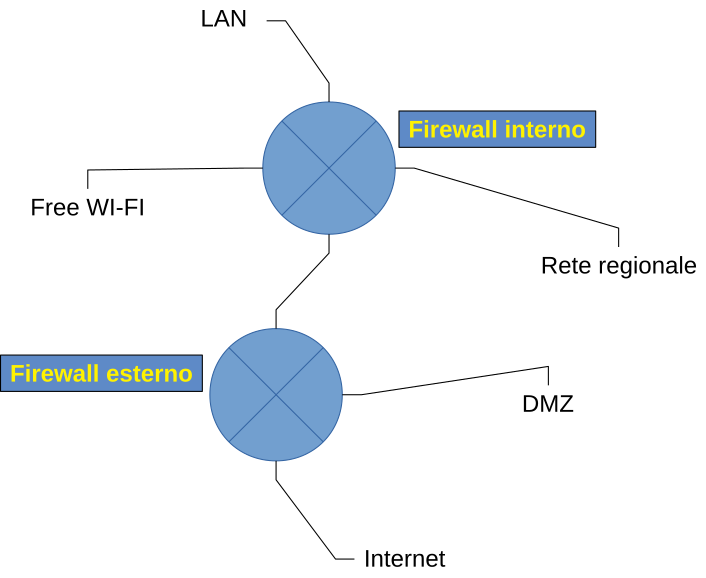
\includegraphics[width=7cm]{rete.png}
	  \caption{Schema delle reti e dei due firewall}
	  \label{fig:rete}
\end{center}
\end{figure}

In particolare sul firewall esterno sono presenti regole di tipo blacklist per
un diversi insiemi di indirizzi, che viene aggiornato
periodicamente (ogni 5 minuti).  Le liste di indirizzi provengono da:

\begin{itemize}
    \item \href{https://iplists.firehol.org/?ipset=firehol\_level1}{''FireHol
	Level1''}\footnote{https://iplists.firehol.org/?ipset=firehol\_level1} (oltre
	7000 sottoreti),
    \item \href{https://ransomwaretracker.abuse.ch/downloads/RW\_IPBL.txt}{''Ransomware
	Tracker}\footnote{https://ransomwaretracker.abuse.ch/downloads/RW\_IPBL.txt}
	(circa 400 indirizzi)
    \item {\em fail2ban} su ssh: blacklist auto-generata in base ai tentativi
	falliti di connessione via ssh (circa 9000 indirizzi al momemnto)
    \item lista di indirizzi di botnet autoprodotta da script che analizzano
	tentativi di bruteforce tipicamente su servizi di posta (oltre 12.000
	indirizzi)
\end{itemize}
 
Si tratta quindi di oltre 20 mila regole.

Il firewall interno ha la particolarità di dover gestire le regole del {\em
captive portal}: si tratta di abilitare il traffico verso internet dei
dispositivi wireless di coloro che si sono autenticati fornando il numero di
telefono e ricevendo un codice di accesso via SMS.  Il sistema di
abilitazione, da me realizzato con la collaborazione di un collega, agisce
classificando i pacchetti in base al mac address: i pacchetti con mac adddress
abilitato vengono inoltrati regolarmente, i rimanenti vengono marcati
(l'associazione del valore al pacchetto è realizzata all'interno del kernel,
il pacchetto resta inalterato) e successivamente una regola nella catena di
inoltro devia il pacchetto verso il sito del captive portal che propone la
registrazione.

Non avendo specificato termini di scadenza la lista di mac address non
decresce mai, ad esempio al momento sono presenti oltre 23 mila indirizzi mac.

\section{Problemi dell'infrastruttura}

Nella sezione precedente ho messo in evidenza gli insiemi di indirizzi e le
loro dimensioni perché sono tali insiemi quelli che hanno evidenziato, ad un
certo punto nell'arco del 2017, alcune carenze della soluzione implementata.

Inizialmente, infatti, per ogni indirizzo era prevista una regola di tipo {\em
REJECT}; ciò significa che prima di poter classificare ogni singolo pacchetto,
a parte ovviamente quelli subito accettati in virtù di regole relative a
traffico {\em REALTED/ESTABLISHED}.  Questo approccio basato su una regola
per ogni indirizzo risulta essere non efficace, superata una certa
soglia\footnote{nella configurazione hardware da me utilizzata questo limite
risultava essere intorno a cira 15 mila regole} risultava evidente il carico
del server Linux tanto che risultavano anche rallentati l'accesso via ssh e
l'esecuzione di comandi.

Come accennato in precedenza iptables non prevede strutture dati quali i {\em
set}, ma un framework esterno, {\em ipset}, fornisce questa funzionalità
permettendo di ridurre decine di migliaia di regole ad un unica regola (nello
specifico una regola per ogni insieme).

I problemi dovuti all'eccessivo numero di regole li ho quindi risolti
introducendo l'uso di ipset su entrambe i firewall.  Nel caso del firewall
interno è stato anche necessario aggiornare il kernel per poter generare set
contenenti mac address in quanto questa funzionalità non è stata sempre
presente.

L'introduzione di ipset ha richiesto, oltre alla modifica della configurazione
dei due firewall, anche le revisione del codice del captive portal e dei
programmi di generazione di black list.

\section{Opportunità di migrazione a nftables}

L'uso di ipset ha risolto i problemi, tuttavia mi sono chiesto se non fosse il
caso di iniziare a prevedere la migrazione a nftables.

Come accennato in precedenza, nftables si propone come framework completamente
nuovo, più che come evoluzione di iptables: il codice kernel space è stato
interamente riscritto, eliminando le ridondanze, e l'interfaccia di
configurazione è diventata un vero e proprio linguaggio di programmazione a
differenza di iptables dove ogni regola viene inserita da un commando con
relativi argomenti.

Un semplice esempio di configurazione per un server web potrebbe essere
questo:

\lstinputlisting[caption=Semplice esempio per server web, style=customc]{nftables-web.conf}

%\begin{lstlisting}
%$ sudo iptables -A INPUT -m conntrack --ctstate ESTABLISHED,RELATED -j ACCEPT
%\end{lstlisting}

\chapter{}
